%%%%%%%%%%%%%%%%%%%%%%%%%%%%%%%%%%%%%%%%%%%%%%%%%%%%%%%%%%%
% --------------------------------------------------------
% Tau
% LaTeX Template
% Version 2.4.3 (01/09/2024)
%
% Author: 
% Guillermo Jimenez (memo.notess1@gmail.com)
% 
% License:
% Creative Commons CC BY 4.0
% --------------------------------------------------------
%%%%%%%%%%%%%%%%%%%%%%%%%%%%%%%%%%%%%%%%%%%%%%%%%%%%%%%%%%%

\documentclass[9pt,a4paper,twoside]{tau-class/tau}
\usepackage[english]{babel}

%----------------------------------------------------------
% TITLE
%----------------------------------------------------------

\journalname{Xarxes Neuronals i Aprenentatge Profund}
%% TODO: Optional, you can set a fancier title if you like
\title{SmallResNet sobre CIFAR-100}

%----------------------------------------------------------
% AUTHORS, AFFILIATIONS AND PROFESSOR
%----------------------------------------------------------

%% TODO: Set your names here
\author[a,1]{Natan Sisoev}

%----------------------------------------------------------

\affil[a]{1706198}

%----------------------------------------------------------
% FOOTER INFORMATION
%----------------------------------------------------------

\institution{Universitat Autònoma de Barcelona}
\footinfo{Entrega 1}
\theday{\today}
\course{XNAP}

%----------------------------------------------------------
% TIKZ: Paleta de colors i macros per al diagrama
%----------------------------------------------------------

\definecolor{Corange}{RGB}{215,148,55}
\definecolor{Cdark}{RGB}{155,75,15}
\definecolor{Cblue}{RGB}{110,162,208}
\definecolor{Cpurp}{RGB}{148,108,182}
\definecolor{Cadd}{RGB}{70,168,128}
\definecolor{Carrow}{RGB}{48,112,102}

% \fmap{x}{channels}{size}{color}{name}
\newcommand{\fmap}[5]{%
    \def\fw{#2/30}%
    \def\fh{#3/10}%
    \def\fd{#3/30}%
    \def\fblx{#1}%
    \def\fbly{3.2/2 - \fh/2 - \fd/2}%
  \fill[#4!62!black]
    (\fblx+\fw,     \fbly)                      --
    (\fblx+\fw+\fd, \fbly+\fd)                  --
    (\fblx+\fw+\fd, \fbly+\fd+\fh)              --
    (\fblx+\fw,     \fbly+\fh)                  -- cycle;
  \fill[#4!52!white]
    (\fblx,         \fbly+\fh)                  --
    (\fblx+\fw,     \fbly+\fh)                  --
    (\fblx+\fw+\fd, \fbly+\fh+\fd)              --
    (\fblx+\fd,     \fbly+\fh+\fd)              -- cycle;
  \fill[#4]
    (\fblx,   \fbly)   -- (\fblx+\fw, \fbly)    --
    (\fblx+\fw,\fbly+\fh) -- (\fblx,  \fbly+\fh) -- cycle;
  \draw[black!48, line width=0.28pt]
    (\fblx,\fbly) -- (\fblx+\fw,\fbly) --
    (\fblx+\fw,\fbly+\fh) -- (\fblx,\fbly+\fh) -- cycle;
  \draw[black!48, line width=0.28pt]
    (\fblx+\fw,\fbly) -- (\fblx+\fw+\fd,\fbly+\fd) --
    (\fblx+\fw+\fd,\fbly+\fd+\fh) -- (\fblx+\fw,\fbly+\fh) -- cycle;
  \draw[black!48, line width=0.28pt]
    (\fblx,\fbly+\fh) -- (\fblx+\fw,\fbly+\fh) --
    (\fblx+\fw+\fd,\fbly+\fh+\fd) -- (\fblx+\fd,\fbly+\fh+\fd) -- cycle;
  \node[font=\fontsize{5.5}{6}\selectfont, inner sep=0.8pt, below]
    at (\fblx+\fw/2, \fbly) {#2};
  \node[font=\fontsize{5.5}{6}\selectfont, inner sep=0.8pt, below, yslant=1]
    at (\fblx+\fw+\fd/2, \fbly+\fd/2+\fh*0.9) {#3$\times$#3};
  \coordinate (#5-back)  at (\fblx,           \fbly+\fh/2+\fd/2);
  \coordinate (#5-front) at (\fblx+\fw+\fd/2, \fbly+\fh/2+\fd/2);
}

\newcommand{\fmapFC}[5]{%
    \def\fw{#2/30}%
    \def\fh{1/10}%
    \def\fd{#3/30}%
    \def\fblx{#1}%
    \def\fbly{3.2/2 - \fh/2 - \fd/2}%
  \fill[#4!62!black]
    (\fblx+\fw,\fbly)              -- (\fblx+\fw+\fd,\fbly+\fd)         --
    (\fblx+\fw+\fd,\fbly+\fd+\fh) -- (\fblx+\fw,\fbly+\fh)             -- cycle;
  \fill[#4!52!white]
    (\fblx,\fbly+\fh)              -- (\fblx+\fw,\fbly+\fh)             --
    (\fblx+\fw+\fd,\fbly+\fh+\fd) -- (\fblx+\fd,\fbly+\fh+\fd)         -- cycle;
  \fill[#4]
    (\fblx,\fbly) -- (\fblx+\fw,\fbly) --
    (\fblx+\fw,\fbly+\fh) -- (\fblx,\fbly+\fh) -- cycle;
  \draw[black!48, line width=0.28pt]
    (\fblx,\fbly) -- (\fblx+\fw,\fbly) --
    (\fblx+\fw,\fbly+\fh) -- (\fblx,\fbly+\fh) -- cycle;
  \draw[black!48, line width=0.28pt]
    (\fblx+\fw,\fbly) -- (\fblx+\fw+\fd,\fbly+\fd) --
    (\fblx+\fw+\fd,\fbly+\fd+\fh) -- (\fblx+\fw,\fbly+\fh) -- cycle;
  \draw[black!48, line width=0.28pt]
    (\fblx,\fbly+\fh) -- (\fblx+\fw,\fbly+\fh) --
    (\fblx+\fw+\fd,\fbly+\fh+\fd) -- (\fblx+\fd,\fbly+\fh+\fd) -- cycle;
  \node[font=\fontsize{5.5}{6}\selectfont, inner sep=0.8pt, below]
    at (\fblx+\fw/2, \fbly) {#2};
  \node[font=\fontsize{5.5}{6}\selectfont, inner sep=0.8pt, below, yslant=1]
    at (\fblx+\fw+\fd/2, \fbly+\fd/2+\fh*0.9) {#3};
  \coordinate (#5-back)  at (\fblx+\fd/2,       \fbly+\fh/2+\fd/2);
  \coordinate (#5-front) at (\fblx+\fw+\fd/2,   \fbly+\fh/2+\fd/2);
}

\newcommand{\addnode}[3]{%
  \filldraw[fill=Cadd!82, draw=black!55, line width=0.45pt]
    (#1,#2) circle (0.185);
  \draw[white, line width=1.15pt]
    (#1-0.12,#2) -- (#1+0.12,#2)
    (#1,#2-0.12) -- (#1,#2+0.12);
  \coordinate (#3) at (#1, #2);
}
\newcommand{\addnodeSimple}[3]{%
  \filldraw[fill=Cadd!82, draw=black!55, line width=0.45pt]
    (#1,#2) circle (0.185);
  \coordinate (#3) at (#1, #2);
}

%----------------------------------------------------------
% ABSTRACT AND KEYWORDS
%----------------------------------------------------------

\begin{abstract}
    Aquest treball presenta \textit{SmallResNet}, una xarxa neuronal convolucional lleugera per a la classificació d'imatges del dataset \textbf{CIFAR-100}. L'arquitectura utilitza blocs residuals de dues convolucions $3{\times}3$ amb normalització per \textit{batch} i connexions de salt, amb ~107K paràmetres.  
    S'han aplicat tècniques d'augmentació de dades (\textit{TrivialAugmentWide}, \textit{CutMix}, \textit{MixUp}) i regularització (\textit{dropout}, decaïment de pesos, \textit{label smoothing}), amb \textit{Cosine Annealing} per al \textit{learning rate}. L'entrenament es va realitzar eficientment a la plataforma \textit{Modal}, explorant diverses estratègies sense restriccions de temps.  
    El model final aconsegueix un \textbf{Top-1 Accuracy del 53\%} després de 300 èpoques, amb marge de millora mitjançant \textit{Cosine Annealing warm restarts}.
\end{abstract}

%----------------------------------------------------------

\keywords{Xarxes neuronals convolucionals, Blocs residuals, Classificació d'imatges,
          Aprenentatge profund, ResNet, CIFAR-100}

%----------------------------------------------------------

\begin{document}
    \maketitle
    \thispagestyle{firststyle} \tauabstract
    \tableofcontents
    \linenumbers

%----------------------------------------------------------

\section{Introducció}

    El dataset \textbf{CIFAR-100} conté 60.000 imatges de $32{\times}32$ píxels distribuïdes
    en 100 classes, amb 50.000 imatges d'entrenament i 10.000 de test. L'objectiu d'aquest
    treball és desenvolupar una xarxa neuronal convolucional eficient que pugui classificar
    les imatges amb un nombre reduït de paràmetres sense sacrificar massa rendiment.
    
    S'ha optat per una arquitectura basada en \textit{ResNet}~\cite{he2016deep} per diversos motius:
    \begin{itemize}
        \item Els blocs residuals permeten el flux estable del gradient, evitant problemes de
              \textit{vanishing gradient} en xarxes amb profunditat moderada.
        \item La connexió de salt (\textit{shortcut}) permet una aprenentatge més ràpid i estable
              amb menys paràmetres.
        \item ResNet ha demostrat ser una arquitectura versàtil i efectiva per a classificació
              d'imatges en múltiples escales, fet que facilita l'adaptació a imatges petites
              com les de CIFAR-100.
    \end{itemize}
    
    L'arquitectura resultant, anomenada \textit{SmallResNet}, està optimitzada per maximitzar
    l'\textit{accuracy} tot mantenint el nombre total de paràmetres per sota de 110K.
    A més, permet explorar fàcilment diferents estratègies d'augmentació i regularització
    per millorar la generalització del model.

\section{Metodologia}
    \subsection{Preprocessament i Augmentació}
    
        Per millorar la generalització i reduir l'\textit{overfitting}, s'han aplicat les següents tècniques
        d'augmentació de dades durant l'entrenament:
        
        \begin{itemize}
            \item \textbf{TrivialAugmentWide}~\cite{muller2021trivialaugment}: aplica una transformació
                  aleatòria per imatge escollida uniformement d'un conjunt ampli de polítiques
                  (rotació, translació, canvi de color, etc.), sense necessitat de tuning.
            \item \textbf{RandomCrop} i \textbf{RandomHorizontalFlip}: transformacions geomètriques bàsiques
                  que augmenten la variabilitat posicional de les imatges.
            \item \textbf{RandomErasing}: elimina aleatòriament rectangles de la imatge per forçar
                  el model a aprendre característiques més robustes.
        \end{itemize}
        
        Durant la fase de validació, només s'aplica la normalització estàndard de CIFAR-100:
        $\mu = (0.507, 0.487, 0.441)$, $\sigma = (0.267, 0.256, 0.276)$.
        
        Cal destacar que alguns intents amb augmentació agressiva i entrenament més curt van mostrar
        una divergència prematura entre les corbes de \textit{train} i \textit{test}, suggerint que
        necessitaríem més èpoques per a generalitzar correctament. També s'han explorat entrenaments
        més enllà de $T_{\max}=100$ del planificador CosineAnnealingLR, amb caiguda de l'\textit{accuracy}
        després de 100 èpoques (vegeu Annex~\ref{sec:annex_failed_attempts} per als detalls i figures dels intents previs).
        

    \subsection{Arquitectura del model}

        S'ha implementat una xarxa \textbf{SmallResNet} basada en blocs residuals lleugers,
        cada un amb dues convolucions $3{\times}3$, normalització per \textit{batch} i activació ReLU.
        Quan hi ha un canvi de canals o de resolució espacial (\textit{stride} $>$ 1), s'utilitza una
        convolució $1{\times}1$ com a \textit{projection shortcut}; en cas contrari, la connexió de
        salt és l'identitat.
        
        L'estructura del model és la següent:
        
        \begin{itemize}
            \item \textbf{Stem:} Conv2d(3$\to$8, $3{\times}3$) + BatchNorm + ReLU
            \item \textbf{Stage 1:} 2 blocs residuals, 16 canals, resolució $32{\times}32$
            \item \textbf{Stage 2:} 2 blocs residuals, 32 canals, resolució $16{\times}16$
            \item \textbf{Stage 3:} 1 bloc residual, 64 canals, resolució $8{\times}8$
            \item \textbf{Cap:} AdaptiveAvgPool2d(1) + Dropout(0.3) + Linear(64$\to$100)
        \end{itemize}
        
        El nombre total de paràmetres entrenables és $\approx 107\text{K}$.
        
        \noindent
        La Figura~\ref{fig:arch} mostra el diagrama complet de l'arquitectura.

        \begin{figure*}[ht]
        \centering
        \begin{tikzpicture}[
          >=Stealth,
          arr/.style     = {draw=Carrow, ->, line width=0.90pt, shorten >=1pt},
          skiparc/.style = {draw=Carrow, ->, line width=0.75pt},
          idskip/.style  = {draw=Carrow, ->, line width=0.75pt, dashed},
          lbl/.style     = {font=\fontsize{5.5}{6}\selectfont, inner sep=0.8pt},
          slbl/.style    = {font=\fontsize{6.5}{7}\selectfont\bfseries,
                            inner sep=0.8pt, text=black!65},
        ]
        
        % ── Imatge d'entrada ────────────────────────────────────────────────
        \fmap{0}{3}{32}{Corange}{image}
        \node[slbl] at (0.5+3/60+32/60, 4) {Entrada};
        
        % ── Stem: Conv(3→8) ─────────────────────────────────────────────────
        \fmap{1}{8}{32}{Corange}{stem}
        \draw[arr] (image-front) -- (stem-back);
        \node[slbl] at (1.55+8/60+32/60, 4) {Stem};
        \addnodeSimple{2.3}{1.6}{afterStem}
        
        \draw[arr] (stem-front) -- (afterStem);
        
        % ── Stage 1: 2 blocs residuals, 16ch, 32×32 ─────────────────────────
        \fmap{2.8}{16}{32}{Corange}{stage1a}
        \fmap{3.7}{16}{32}{Corange}{stage1b}
        \addnode{5.4}{1.6}{sum1}
        
        \draw[arr] (afterStem) -- (stage1a-back);
        \draw[arr] (stage1b-front) -- (sum1);
        
        \draw[skiparc]
          (afterStem)
            .. controls ($(afterStem)-(0,1.5)$) and ($(sum1)-(0,1.5)$) ..
          (sum1);
        \node[lbl, text=Carrow, below] at ($(afterStem)!0.5!(sum1)-(0,1.5)$) {identitat};
        
        \node[slbl] at (4.6, 4) {Stage 1};
        
        % ── Stage 2: 2 blocs residuals, 32ch, 16×16 ─────────────────────────
        \fmap{5.8}{32}{16}{Corange}{stage2a}
        \fmap{7}{32}{16}{Corange}{stage2b}
        \addnode{9}{1.6}{sum2}
        
        \draw[arr] (sum1) -- (stage2a-back);
        \draw[arr] (stage2b-front) -- (sum2);
        
        \draw[skiparc]
          (sum1)
            .. controls ($(sum1)-(0,1.3)$) and ($(sum2)-(0,1.3)$) ..
          (sum2);
        \node[lbl, text=Carrow, below] at ($(sum1)!0.5!(sum2)-(0,1.3)$) {proj. $1{\times}1$};
        
        \node[slbl, below] at (7.5,4) {Stage 2};
        
        % ── Stage 3: 1 bloc residual, 64ch, 8×8 ─────────────────────────────
        \fmap{9.5}{64}{8}{Corange}{stage3a}
        \addnode{12.5}{1.6}{sum3}
        
        \draw[arr] (sum2) -- (stage3a-back);
        \draw[arr] (stage3a-front) -- (sum3);
        
        \draw[skiparc]
          (sum2)
            .. controls ($(sum2)-(0,1.1)$) and ($(sum3)-(0,1.1)$) ..
          (sum3);
        \node[lbl, text=Carrow, below] at ($(sum2)!0.5!(sum3)-(0,1.1)$) {proj. $1{\times}1$};
        
        \node[slbl, below] at (10.7,4) {Stage 3};
        
        % ── Cap: AvgPool + Dropout + FC ─────────────────────────────────────
        \fmap{13}{64}{1}{Cblue}{pool}
        \draw[arr] (sum3) -- (pool-back);
        \node[slbl, below] at (13.8, 4) {AvgPool};
        
        \fmapFC{15}{1}{100}{Cpurp}{fc}
        \draw[arr] (pool-front) -- (fc-back);
        \node[slbl, below] at (17, 4) {FC(100)};
        
        % ── Títol ────────────────────────────────────────────────────────────
        \node[font=\normalsize\bfseries, below] at (9,-0.5)
          {\textsc{SmallResNet}};
        
        \end{tikzpicture}
        \caption{Diagrama de l'arquitectura \textit{SmallResNet}. Cada cub representa un mapa de característiques (amplada $\propto$ canals, alçada $\propto$ resolució espacial). Els nodes verd-clar ($\oplus$) indiquen la suma element a element entre la branca principal i la connexió de salt. Les fletxes indiquen connexions identitat i de projecció $1{\times}1$.}
        \label{fig:arch}
        \end{figure*}

    \subsection{Entrenament}

        L'entrenament s'ha realitzat utilitzant les següents configuracions:
        
        \begin{itemize}
            \item \textbf{Funció de pèrdua:} CrossEntropyLoss amb \textit{label smoothing} $\epsilon = 0.1$ (per la gran quantitat de classes que hi ha).
            \item \textbf{Optimitzador:} SGD amb $lr=0.1$, momentum $0.9$, decaïment de pesos $1{\times}10^{-3}$ i Nesterov activat.
            \item \textbf{Planificador:} \textit{CosineAnnealingLR} amb $T_{\max}=300$ èpoques (per la transició suau entre \textit{learning rate} màxim i mínim).
            \item \textbf{Mida de \textit{batch}:} 128.
            \item \textbf{Dispositiu:} GPU si està disponible
        \end{itemize}
        
        Es van monitoritzar la pèrdua i el \textit{Top-1 Accuracy} durant l'entrenament.
        
\section{Resultats}

    Els resultats es mostren mitjançant les mètriques principals obtingudes al conjunt de test després de 300 èpoques: la funció de pèrdua, \textit{Top-k Accuracy} per diversos valors de \textit{k}, el \textit{F1} score i la mètrica \textit{d} (entesa com la distància al punt \((0,1)\) del model en un espai de l'\textit{accuracy} contra el nombre de paràmetres (en centenars de milers).
    
    \begin{table}[h!]
    \centering
    \begin{tabular}{l c}
    \hline
    \textbf{Mètrica} & \textbf{Valor} \\
    \hline
    Test Loss & 1.8532 \\
    Top-1 Accuracy & 52.95\% \\
    Top-2 Accuracy & 67.30\% \\
    Top-3 Accuracy & 75.07\% \\
    Top-4 Accuracy & 79.84\% \\
    Top-5 Accuracy & 83.25\% \\
    F1 Score (macro) & 0.5139 \\
    d metric & 1.1588 \\
    \hline
    \end{tabular}
    \caption{Mètriques principals del model SmallResNet al conjunt de test.}
    \label{tab:metrics}
    \end{table}

    En la Figura~\ref{fig:history_final} s'observa que després de 300 èpoques la corba de validació es torna més estable, degut a la reducció gradual del \textit{learning rate} amb Cosine Annealing. La corba d'entrenament mostra un lleuger increment constant, suggerint que el model podria beneficiar-se de més èpoques d'entrenament, o possiblement de \textit{warm restarts} per sortir dels mínims locals més ràpidament.

    \begin{figure}[h!]
        \centering
        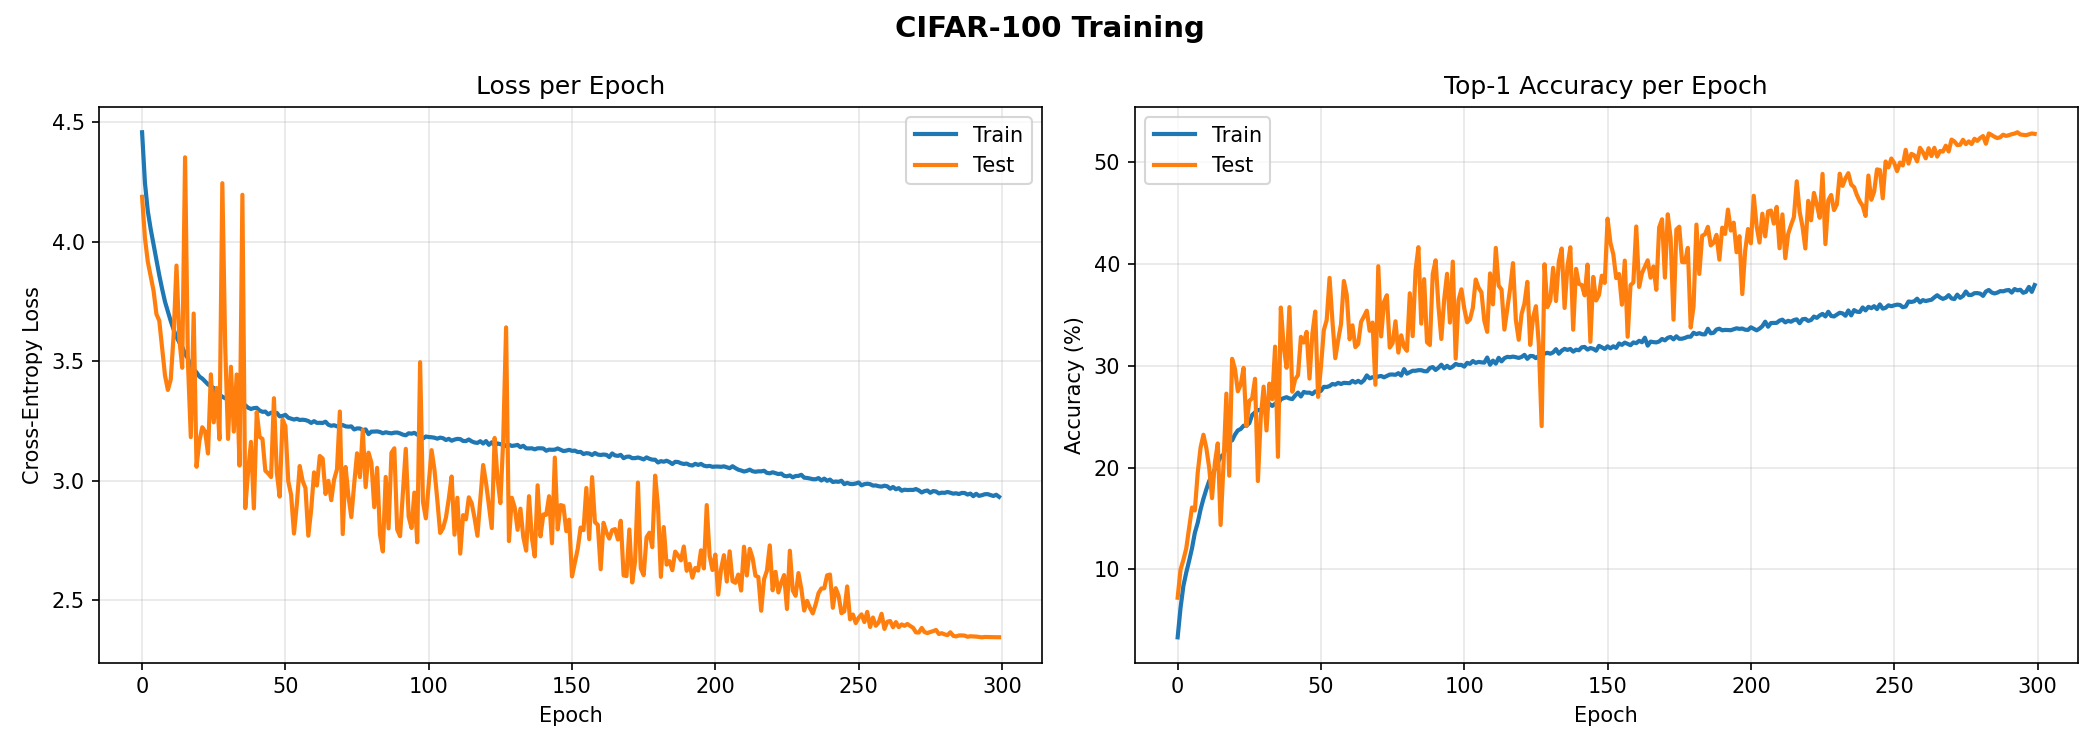
\includegraphics[width=0.5\textwidth]{plots/history_final.png}
        \caption{Història d'entrenament final amb $T_{\max}=300$. Mostra estabilització de l'accuracy i convergència del model SmallResNet.}
        \label{fig:history_final}
    \end{figure}
    
    \noindent
    La corba de \textit{Top-k Accuracy} es mostra a la Figura~\ref{fig:topk}. S'observa que la major part de les prediccions correctes es concentren en les primeres posicions, ja que la corba és més creixent per \textit{k}'s petits.
    
    \begin{figure}[h!]
        \centering
        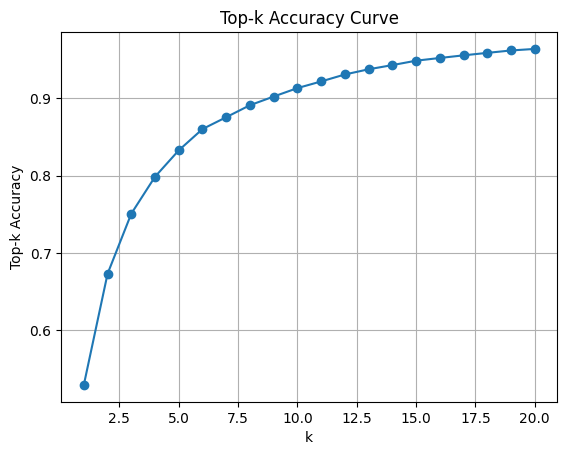
\includegraphics[width=0.35\textwidth]{plots/top_k.png}
        \caption{Corba de \textit{Top-k Accuracy} del model SmallResNet.}
        \label{fig:topk}
    \end{figure}

\section{Conclusions}
    
    \begin{itemize}
        \item \textit{SmallResNet} aconsegueix Top-1 Accuracy del 52.95\% amb aproximadament 107K paràmetres, demostrant que arquitectures lleugeres poden ser efectives en tasques de classificació amb moltes classes.
        \item La combinació d'augmentació de dades (TrivialAugmentWide) i regularització (dropout, decaïment de pesos, label smoothing) ha ajudat per millorar la generalització en conjunts de dades petits com CIFAR-100.
        \item Els blocs residuals faciliten l'aprenentatge estable i permeten entrenaments més llargs sense degradació significativa del gradient.
        \item L'estratègia de \textit{Cosine Annealing} amb $T_{\max}=300$ contribueix a una convergència estable; les corbes finals mostren que la validació es manté estable quan el \textit{learning rate} és molt baix, suggerint possibilitat de més aprenentatge amb \textit{warm restarts} o entrenament addicional.
    \end{itemize}

\appendix

\section{Repositori GitHub}
    
    El codi font complet i les dades del projecte es troben disponibles al repositori GitHub:  
    
    \begin{itemize}
        \item \textbf{Repositori:} \url{https://github.com/natansisoev/CIFAR-100-Classification}
        \item Conté:
        \begin{itemize}
            \item Scripts per a entrenament i avaluació (\texttt{models/train.py}, \texttt{notebooks/}).
            \item Codi del model \textit{SmallResNet} (\texttt{models/smallresnet.py}).
            \item Funcions d'augmentació i utilitats de dataset (\texttt{data/}).
            \item Arxius de plots i models guardats (\texttt{artifacts/}).
            \item Configuracions i dependències (\texttt{configs/config.py}, \texttt{requirements.txt}).
        \end{itemize}
        \item El repositori permet reproduir els experiments, visualitzar els resultats i modificar hiperparàmetres amb facilitat.
    \end{itemize}

\section{Intents previs}
\label{sec:annex_failed_attempts}

Aquest annex descriu intents previs abans de definir la configuració final del model SmallResNet.
    
    \subsection*{Entrenament amb $T_{\max}=100$}
        L'ús del planificador \textit{Cosine Annealing} amb $T_{\max}=100$ i l'entrenament (erroni) un cop passades aquestes èpoques va provocar una caiguda de la \textit{Top-1 Accuracy} significant. Aquest fenomen evidencia que un nombre insuficient d'èpoques pot limitar la convergència, especialment en xarxes residuals que encara necessiten estabilitzar els pesos al llarg de les etapes inicials i mitjanes d'entrenament.
    
    \subsection*{Augmentació agressiva amb CutMix i MixUp}
        L'augmentació agressiva amb CutMix~\cite{yun2019cutmix} i MixUp~\cite{zhang2017mixup} va mostrar una separació important entre les corbes de pèrdua i \textit{accuracy} de \textit{train} i \textit{test}. Tot i que la \textit{Top-1 Accuracy} gairebé arribava al 50\% en 300 èpoques, aquest entrenament curt no és suficient per capturar totes les característiques generals. Aquest efecte és típic quan l'augmentació força el model a aprendre representacions més difícils amb menys temps d'entrenament, indicant que caldrien més èpoques ($T_{\max}$ més llarg) per aprofitar plenament aquestes tècniques.

    \begin{figure}[h!]
        \centering
        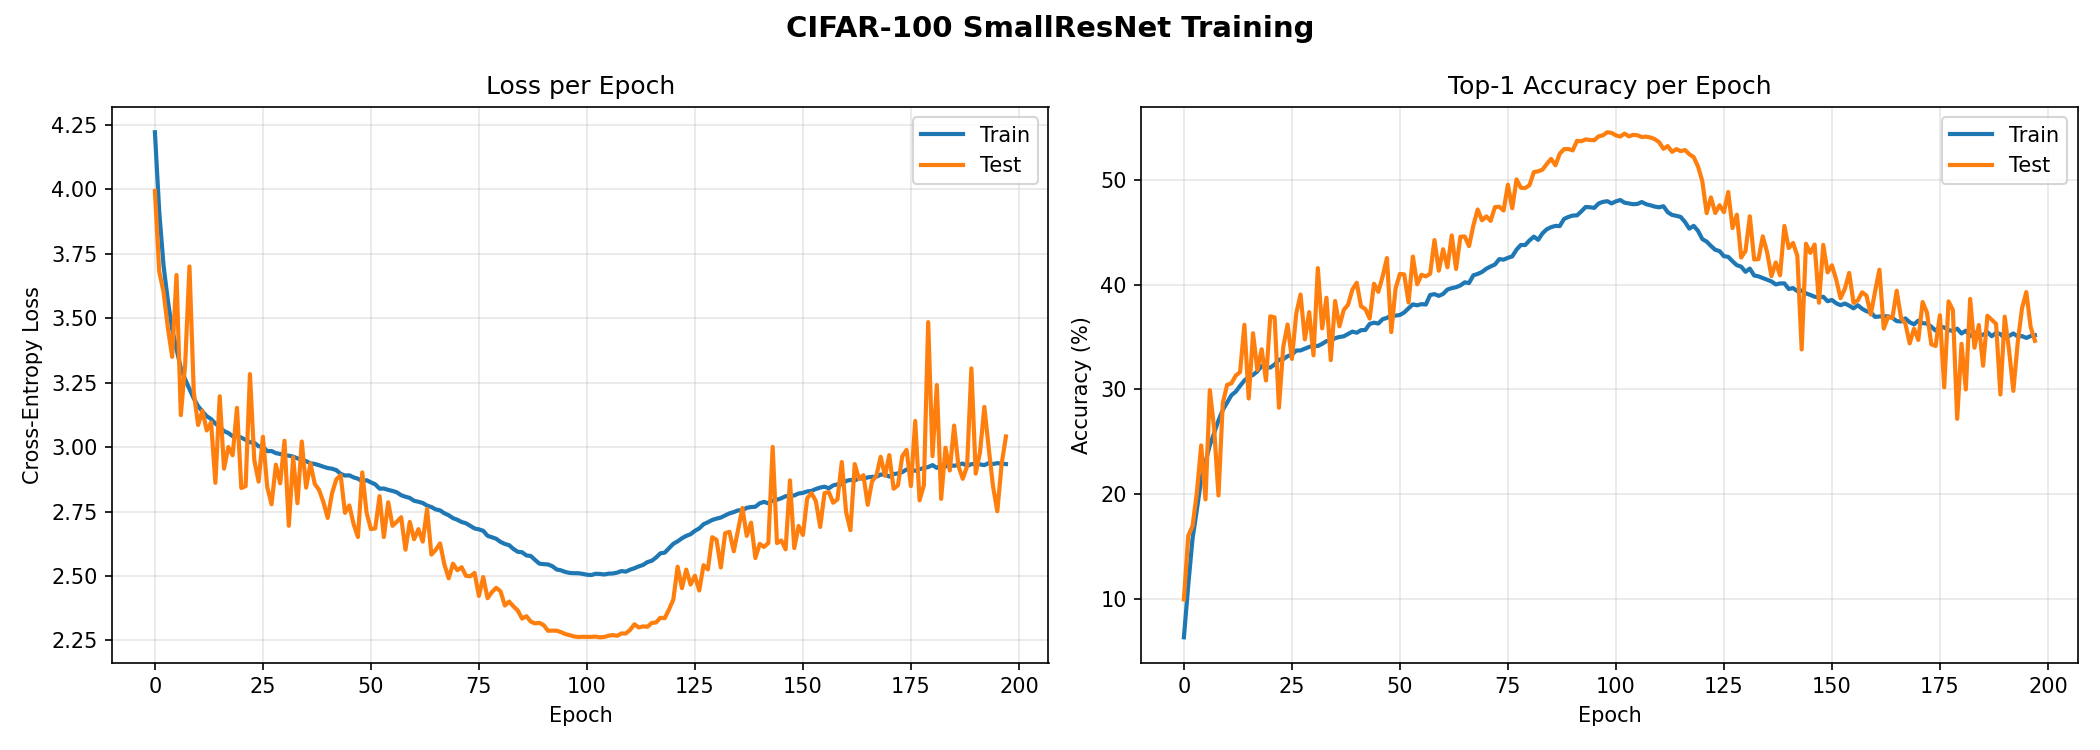
\includegraphics[width=0.475\textwidth]{plots/history_past_cosine.png}
        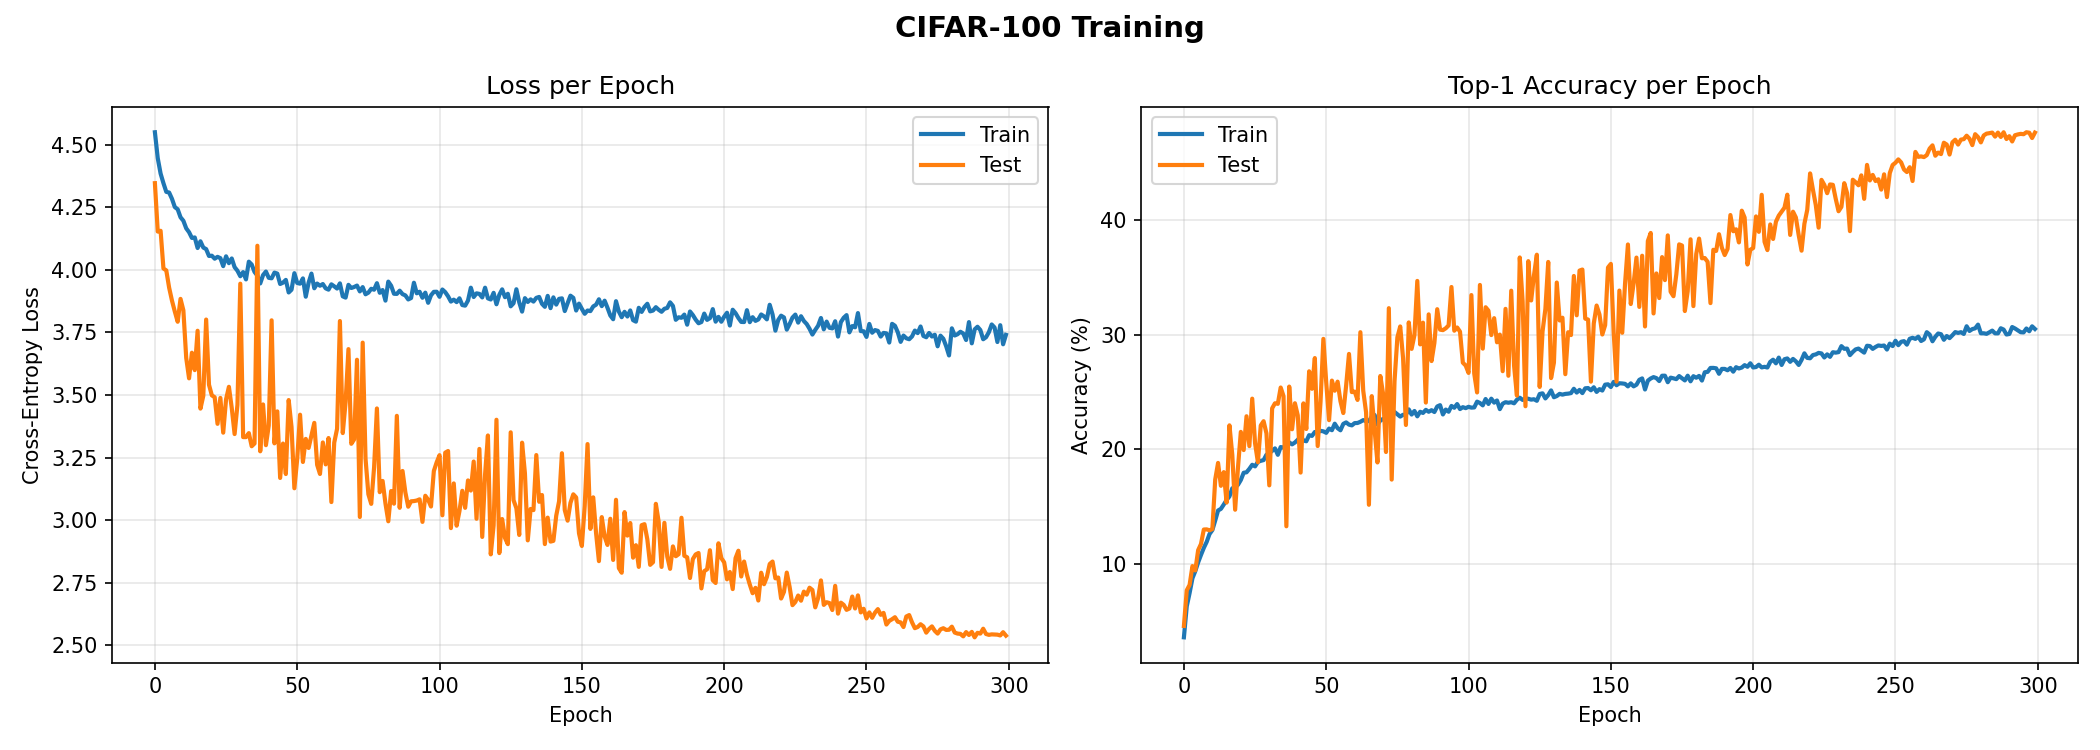
\includegraphics[width=0.475\textwidth]{plots/history_data_augmentation.png}
        \caption{A dalt: entrenament amb $T_{\max}=100$, observant caiguda de l'accuracy. A baix: augmentació agressiva, separació prematura de train i test.}
        \label{fig:failed_attempts}
    \end{figure}
    
    \subsection*{Conclusions dels intents previs}
        Aquests intents mostren la importància de:
        \begin{itemize}
            \item Ajustar correctament el nombre d'èpoques i el planificador de \textit{learning rate} per estabilitzar l'aprenentatge.
            \item Analitzar la interacció entre augmentació de dades i durada d'entrenament: tècniques agressives com CutMix o MixUp poden beneficiar la generalització, però requereixen més temps per convergir.
        \end{itemize}
    
\addcontentsline{toc}{section}{Referències}
    \begin{thebibliography}{10}
    
    \bibitem{he2016deep}
    Kaiming He, Xiangyu Zhang, Shaoqing Ren, and Jian Sun,
    \textit{Deep Residual Learning for Image Recognition},
    arXiv preprint arXiv:1512.03385, 2015.
    
    \bibitem{muller2021trivialaugment}
    Samuel G.\ M\"uller and Frank Hutter,
    \textit{TrivialAugment: Tuning-free Yet State-of-the-art Data Augmentation},
    arXiv preprint arXiv:2103.10158, 2021.
    
    \bibitem{yun2019cutmix}
    Sangdoo Yun, Dongyoon Han, Seong Joon Oh, Sanghyuk Chun, Junsuk Choe, and Youngjoon Yoo,
    \textit{CutMix: Regularization Strategy to Train Strong Classifiers with Localizable Features},
    arXiv preprint arXiv:1905.04899, 2019.
    
    \bibitem{zhang2017mixup}
    Hongyi Zhang, Moustapha Cisse, Yann N.\ Dauphin, and David Lopez-Paz,
    \textit{mixup: Beyond Empirical Risk Minimization},
    arXiv preprint arXiv:1710.09412, 2017.
    
    \end{thebibliography}

\end{document}
